\section[M5: Sirius]{M5: Sirius - grafischer Editor}
\begin{frame}{Sirius - grafischer Editor}
	\vspace{-5mm}
	\begin{columns}
		\column{.5\textwidth}
		\begin{contentblock}{}
			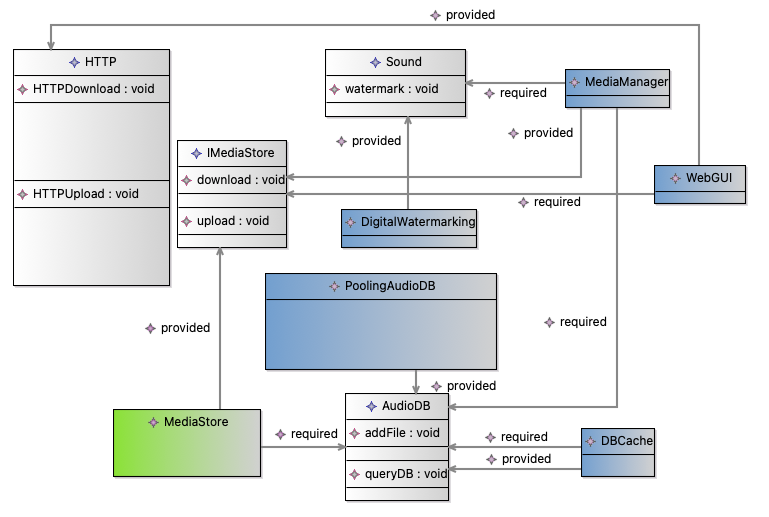
\includegraphics[width=86mm]{figures/sirius.png}
		\end{contentblock}
		\column{.5\textwidth}
		\begin{contentblock}{}
			\begin{itemize}
				\item graues Element: Interface
				\item grünes Element: Composite Component
				\item blaues Element: Component
				\item required Edge: z.B. Component required Interface 
				\item provided Edge: z.B. Component provided Interface
			\end{itemize}
		\end{contentblock}
	\end{columns}
\end{frame}

\begin{frame}{Entwurfsentscheidungen beim grafischen Editor}
	\begin{itemize}
		\item Parameter werden als Liste innerhalb von Signaturblöcken dargestellt
	\end{itemize}
\end{frame}